\documentclass[11pt]{article}
\usepackage[margin=0.75in]{geometry}
\usepackage{amsmath,amsfonts}
\usepackage{enumitem}
\usepackage{tikz}
\usepackage{soul}

\usepackage{multicol}

\newcommand{\ds}{\displaystyle}
\newcommand{\N}{\mathbb{N}}
\newcommand{\R}{\mathbb{R}}
\newcommand{\C}{\mathbb{C}}
\newcommand{\re}{\operatorname{Re}}
\newcommand{\im}{\operatorname{Im}}
\newcommand{\on}{\operatorname}
\newcommand{\Log}{\on{Log}}
\newcommand{\Arg}{\on{Arg}}


\begin{document}
\newcounter{enumCount}
\pagestyle{empty} 
\subsection*{Math 444 - Homework 7 \hfill Name: \underline{\hspace*{2in}}}

\begin{enumerate}


\item In this problem you will evaluate the integral $\ds \int_\gamma |z|^2 \, dz$ where $\gamma(t)$ is the parabola $\gamma(t) = -t + i(t^2-1)$ from $t=-1$ to $t = 1$. 
\begin{enumerate}
\item What are the real and imaginary parts of $|\gamma(t)|^2 \cdot \gamma'(t)$?
\vfill

\item Use the real and imaginary parts above to evaluate $\ds \int_\gamma |z|^2 \, dz$.
\end{enumerate}
\vfill

\item Integrate the function $z - \overline{z}$ on the upper half of the unit circle from $z=1$ to $z=-1$. 
\vfill



%\begin{flushright}
%\begin{tikzpicture}
%\draw[->] (-2,0) -- (2,0);
%\draw[->] (0,-1.5) -- (0,1);
%\draw[very thick,blue] (1,0) -- (1,-1) -- (-1,-1) -- (-1,0);
%\draw[very thick,blue,->] (1,0) -- (1,-1);
%\draw[very thick,blue,->] (1,-1) -- (-1,-1);
%\draw[very thick,blue,->] (-1,-1) -- (-1,0);
%\fill[blue] (1,0) circle (0.05) node[above right,scale=0.6] {1};
%\fill[blue] (1,-1) circle (0.05) node[below right,scale=0.6] {1-i};
%\fill[blue] (-1,-1) circle (0.05) node[below left,scale=0.6] {-1-i};
%\fill[blue] (-1,0) circle (0.05) node[above left,scale=0.6] {-1};
%\end{tikzpicture}
%\end{flushright}

\item Find the length of the path $\gamma(t) = t + \tfrac{2}{3} t^{3/2} i$, $0 \le t \le 3$.  
\vfill 


\newpage

\item Show that $\ds \lim_{n \rightarrow \infty} \left| \int_\gamma \frac{1}{z} \, dz \right|=0$ when $\gamma$ is the horizontal line segment from $1-ni$ to $-1 - ni$. Hint: One way to do this would be to calculate the integral exactly for any $n$. An easier alternative is to use the inequality
$$\left| \int_\gamma f(z) \, dz \right| \le \operatorname{length}(\gamma) \cdot \max_{z \in \text{range}(\gamma)} |f(z)|.$$
\vfill  
\vfill  
\vfill  

\setcounter{enumCount}{\theenumi}
\end{enumerate}

\noindent
Use a computer (I recommend Sympy) to calculate the following integrals.
\begin{enumerate}
\setcounter{enumi}{\theenumCount}
\item $\ds \int_\gamma (\overline{z})^3 \, dz$ on the piecewise path shown below. Hint: in Sympy the complex conjugate function is \verb|conjugate( )|.  You'll need to parameterize each piece separately.  
\begin{flushright}
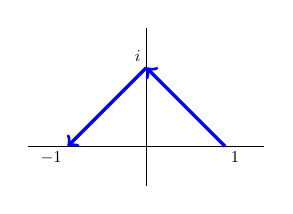
\begin{tikzpicture}
\draw (-1.5,0) -- (1.5,0);
\draw (0,-0.5) -- (0,1.5);
\draw (1.0,0) node[below right,scale=0.6] {$1$};
\draw (-1.0,0) node[below left,scale=0.6] {$-1$};
\draw (0,1.0) node[above left,scale=0.6] {$i$};
\draw[very thick, blue,->] (1,0) -- (0,1);
\draw[very thick, blue,->] (0,1) -- (-1,0);
\end{tikzpicture}
\end{flushright}
\vfill


\item $\ds \int_\gamma (\overline{z})^3 \, dz$ on the piecewise path shown below. %Hint: in Sympy the complex conjugate function is \verb|conjugate( )|.  You'll need to parameterize each piece separately.  
\begin{flushright}
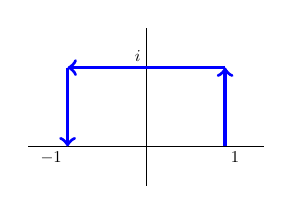
\begin{tikzpicture}
\draw (-1.5,0) -- (1.5,0);
\draw (0,-0.5) -- (0,1.5);
\draw (1.0,0) node[below right,scale=0.6] {$1$};
\draw (-1.0,0) node[below left,scale=0.6] {$-1$};
\draw (0,1.0) node[above left,scale=0.6] {$i$};
\draw[very thick, blue,->] (1,0) -- (1,1);
\draw[very thick, blue,->] (1,1) -- (-1,1);
\draw[very thick, blue,->] (-1,1) -- (-1,0);
\end{tikzpicture}
\end{flushright}
\vfill

%\item Some integrals are too hard to evaluate exactly, even for a computer. But you can always use a Riemann sum to estimate the value numerically.  Use a Riemann sum with $n = 1000$ steps to estimate $\ds \int_\gamma \sin(z) \, dz$ on the spiral path $\gamma(t) = t e^{i t}$ for $0 \le t \le 1$. To calculate the Riemann sum, you can either use
%$$\sum_{k = 1}^n f(z_k) \Delta z_k ~~~~~\text{ or } ~~~~~ \sum_{k = 1}^n f(\gamma(t_k)) \gamma'(t_k) \Delta t.$$ 
%Include your code with your solution for this problem.
%\vfill 

\end{enumerate}


\end{document}
